\chapter{Experimental Results} % (fold)
\label{cha:experiments}

This chapter presents the experimental work completed to validate the actuator dynamics and motion control framework used in simulation. It is important to test walking control strategies on physical hardware directly due to the imperfections in a simulation environment. For example, the contact models used to estimate the ground reaction force is only an approximation. There are also other unmodeled effects which can significantly alter the dynamics of the physical system (i.e. vibrations). The simulations used to demonstrate the proposed 3D FPE walking control strategy in the previous section was designed to account for link side dynamics only. Section~\ref{sec:actuator_model} describes the modifications to account for the actuator dynamics. This modification to the simulations enables a single controller designed in Simulink to target either the simulation environment or the physical hardware using the HIL architecture discussed in Section~\ref{sec:hil_architecture}. The experimental validation for a single actuator and the proposed motion control framework are presented in Sections \ref{sec:1dof_validation} and \ref{sec:motion_control_validation}, respectively. 

\section{Actuator Model} % (fold)
\label{sec:actuator_model}
Thus far, PD control has been applied for each joint in order to track the desired trajectory generated by higher levels of control (Section~\ref{sub:control_strategy}). The control signal $u$ produced at each joint $k$ is provided by (where $k = 1 \ldots n$ is the $k$-th joint of the $n$-DOF system) : 

\begin{equation}
	{u_k} = {K_P}({q_{d_k}} - {q_k}) - {K_D}{\dot q_k}
	\label{eq:pdcontrollaw}
\end{equation} 

Where ${q_{d_k}}$ and ${q_k}$ are the desired and actual angles and ${\dot q_k}$ is the velocity of the $k$-th joint. Constants ${K_P}$ and ${K_D}$ are the porportional and derivative gains of the controller, respectively. In the ideal case, the control signal ${u_k}$ would simply be applied torque ${\tau _k}$ to each joint from $\vtau = \left[\tau _1 \ldots \tau _k \right]$ shown on the right hand side of (\ref{eq:eom1}). However, the actuator dynamics of DC motors used in the development of the 14 DOF bipedal robot must be considered. The motors selected in Section~\ref{sub:final_configurations} are controlled by a voltage control signal $v_{m}$. A second order system is used to model the actuator dynamics and relate the applied torque to the motor voltage $v _m$ \cite{Spong2008}: 

\begin{equation}
	{J_m}{\ddot \Theta _m} + \left( {{B_m} + \frac{{{k_b}{k_m}}}{{{r_a}}}} \right)\dot \Theta _m  = {\tau _m} - \frac{{{\tau _l}}}{{{g_r}}}
	\label{eq:actdyn1}
\end{equation}

Where $\Theta _m$ is the rotor angle, $J_m$ is the motor inertia, $B_m$ is the motor damping, $k_b$ is the back emf or voltage constant, $k_m$ is the torque constant, $r_a$ is the armature resistance, $g_r$ is reduction ratio from the gearhead. The motor torque $\tau _m$ is related to the (link side) load torque $\tau _l$ through the gearing ratio $g_r$. Since the output side of the gearhead is coupled directly to the link, the motor angles are related to the joint angles by: 

\begin{equation}
	{\Theta _{m_k}} = {g _{r_k}} {q _k}
	\label{eq:actdyn2} 
\end{equation}

Similarly, the joint torques in $\vtau$ (\ref{eq:eom1}) are related to the actuator load torques by: 

\begin{equation}
	{\tau _{l_k}} = {\tau _k} 
	\label{eq:actdyn3}
\end{equation}

Furthermore, the electrical characteristics of DC motors relate the motor torque to the applied voltage through the following relationship: 

\begin{equation}
	{\tau _{m_k}} = {k_m} {i_a} = \left( {\frac{{{k_m}}}{{{r_a}}}} \right){v _{m_k}}
	\label{eq:actdyn4}
\end{equation}


Where $i_a$ is the current through the armature wiring. Substituting equations (\ref{eq:actdyn2} - \ref{eq:actdyn4}) back into (\ref{eq:actdyn1}) yields the complete relationship between the $k$-th joint angle, link side torque and the applied motor voltage:

\begin{equation}
	g_r^2{J_m}{\ddot q_k} + g_r^2\left( {{B_m} + \frac{{{k_b}{k_m}}}{{{r_a}}}} \right){\dot q_k} = g_r^{}\left( {\frac{{{k_m}}}{{{r_a}}}} \right){v_k} - {\tau _k}
	\label{eq:actdyn5}
\end{equation}

Note that the drivetrain constants specific to the $k$-th joint are used (i.e. ${J _{m_k}}$, ${B _{m_k}}$, $g _{r_k}$, etc.) in this equation (\ref{eq:actdyn5}). 

Using independent joint control \cite{Sciavicco2001}, each joint $k$ of the system is decoupled from the rest of the system and controlled individually. The control signal for each joint is computed directly from its own reference trajectory, position and velocity. This approach does not account for the coupled dynamics of the overall system described by (\ref{eq:eom1}). To account for this, the link side torques in (\ref{eq:actdyn5}) is treated as a disturbance to the second order system and the motor inertia and damping are modified as follows: 

\begin{equation}
	\begin{array}{l}
		{J_{eff}} = g_r^2{J_m} + {a_{kk}}\\
		{B_{eff}} = g_r^2({B_m} + {k_b}{k_m}/{r_a})
	\end{array}
	\label{eq:actdyn6}
\end{equation}

Where ${J_{eff}}$ and ${B_{eff}}$ are the effective motor inertia and damping \emph{seen} by the joint. The ${a_{kk}}$ in (\ref{eq:actdyn6}) compensates for the inertia of link $k$ by adding the $k$-th diagonal term from the inertia matrix $A(\vec{q})$ in (\ref{eq:eom1}). Substituting back into (\ref{eq:actdyn5}) yields: 

\begin{equation}
	{J_{eff}}{\ddot q_k} + {B_{eff}}{\dot q_k} = g_r^{}\left( {\frac{{{k_m}}}{{{r_a}}}} \right){v_k} - {d_k}
	\label{eq:actdyn7}
\end{equation}

Where ${d_k} = \tau _k$ is the link side torque treated as a disturbance to the system. Taking the control input $u _k$ (\ref{eq:pdcontrollaw}) to be the voltage signal $v _m$ in (\ref{eq:actdyn7}) yields a closed loop controller for independent joint control with actuator dynamics (implemented in Figure~\ref{fig:pdmotorcontroller}).

\begin{figure}[!h]
	\centering
    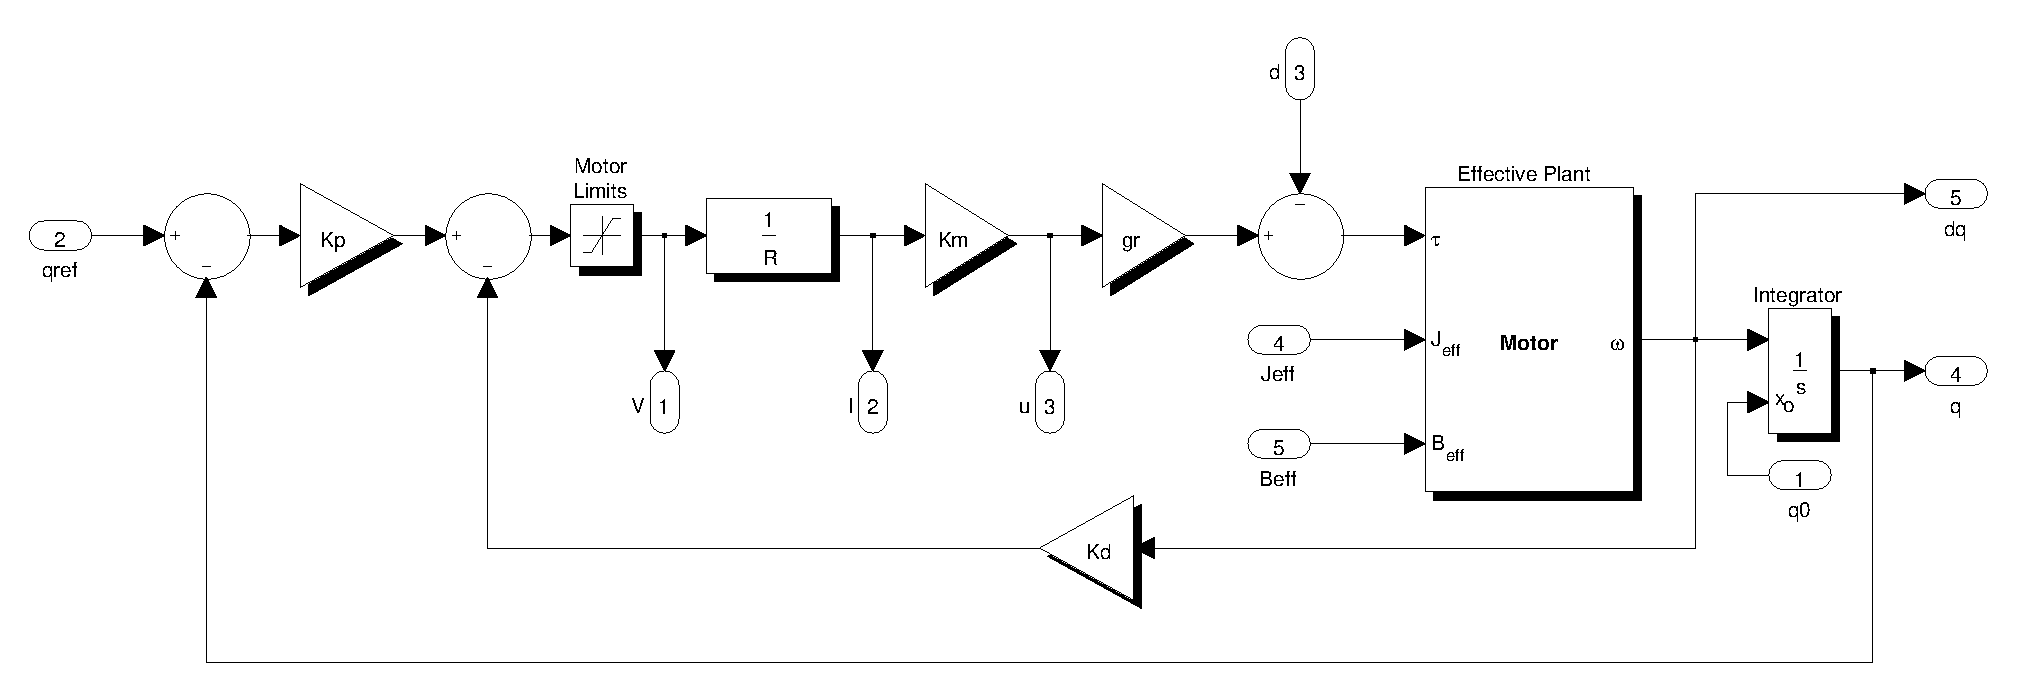
\includegraphics[scale=0.5]{fig/experiments/pdmotorcontroller.eps} 
  	\caption{PD Controller implementation for independent joint control with actuator dynamics.}
	\label{fig:pdmotorcontroller}
\end{figure}

One thing in particular to note is the calculation of $a_{kk}$ in (\ref{eq:actdyn6}). The dynamic simulation package used in Section~\ref{sec:simulations_and_results} is based on Mathwork's Simulink environment and uses the SimMechanics toolbox. Unfortunately, it was found that it is not possible to extract the mass matrix $A(\vec{q})$ symbolically or numerically. Therefore, the following algorithm was used to compute the mass matrix and extract the diagonal terms at each time step: 

\begin{algorithm}[H]
 \SetAlgoLined
 Initialization\;
 Set $\vec{q} = \vec{q}_0$, $\vec{\dot q} = \vec{\dot q}_0$, $\vec{\ddot q} = \vec{0}$\;
 \While{1}{
  Compute $\hat{\vtau}$ using RNE with $\vec{\ddot q} = \vec{0}$\;
  \For{$i = 1$ to $n$}{
  Set $\tilde{\vec{g}} = \vec{0}$, $\mathbf{\tilde{\dot{q}}} = \vec{0}$, $\mathbf{\tilde{\ddot{q_i}}} = 1$, $\mathbf{\tilde{\ddot{q_j}}} = 0$ $[j \ne i]$\;
  Compute $\tilde{\vtau}$ using RNE\;
  Form $i$-th column: $A(\vec{q})_{i} = \tilde{\vtau} - \hat{\vtau}$
  }
  Combine columns to form $A(\vec{q})$\;
  Select diagonal elements of $A(\vec{q})$\;
 }
 \caption{Computing mass matrix diagonal terms with RNE algorithm}
\end{algorithm}

% section actuator_model (end)

\section{HIL Architecture} % (fold)
\label{sec:hil_architecture}
\Incomplete 

\begin{figure}[!h]
	\centering
    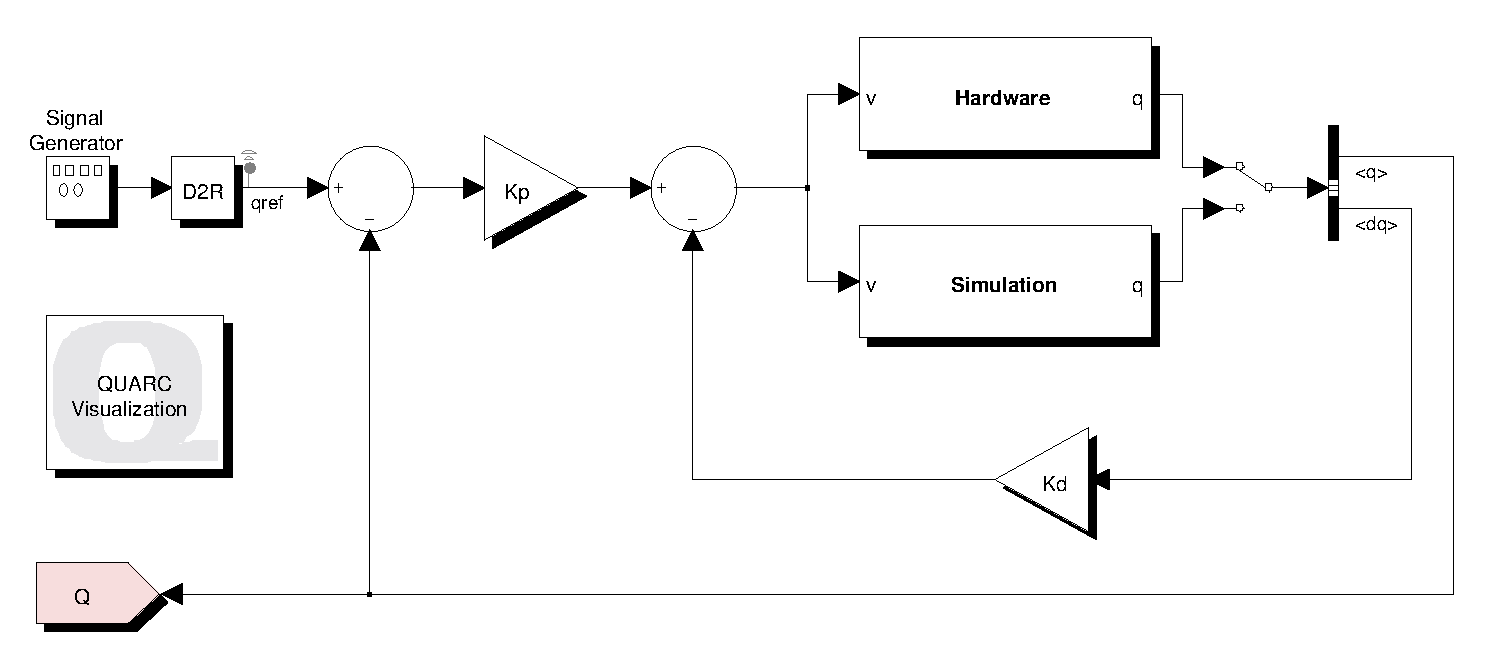
\includegraphics[scale=0.6]{fig/experiments/parallelmodels.eps} 
  	\caption{Parallel models designed to target either simulations or physical hardware with the same controller.}
	\label{fig:parallelmodels}
\end{figure}

\begin{figure}[!h]
	\centering
    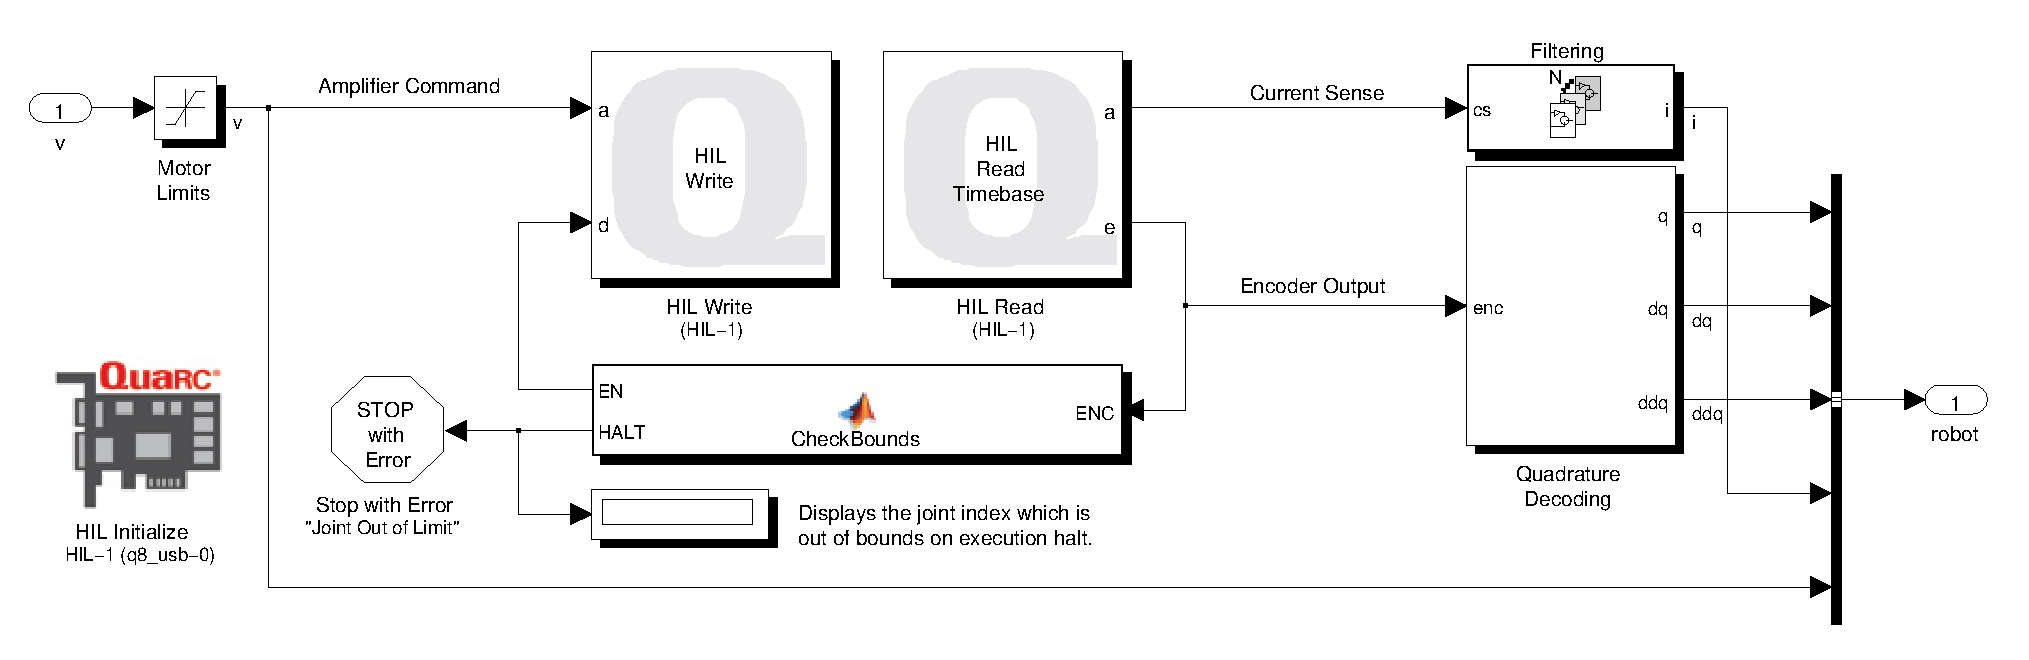
\includegraphics[scale=0.45]{fig/experiments/hilmodel.eps} 
  	\caption{HIL subsystem from Figure~\ref{fig:parallelmodels} used to target physical hardware with voltage control signal.}
	\label{fig:hilmodel}
\end{figure}

\begin{figure}[!h]
	\centering
    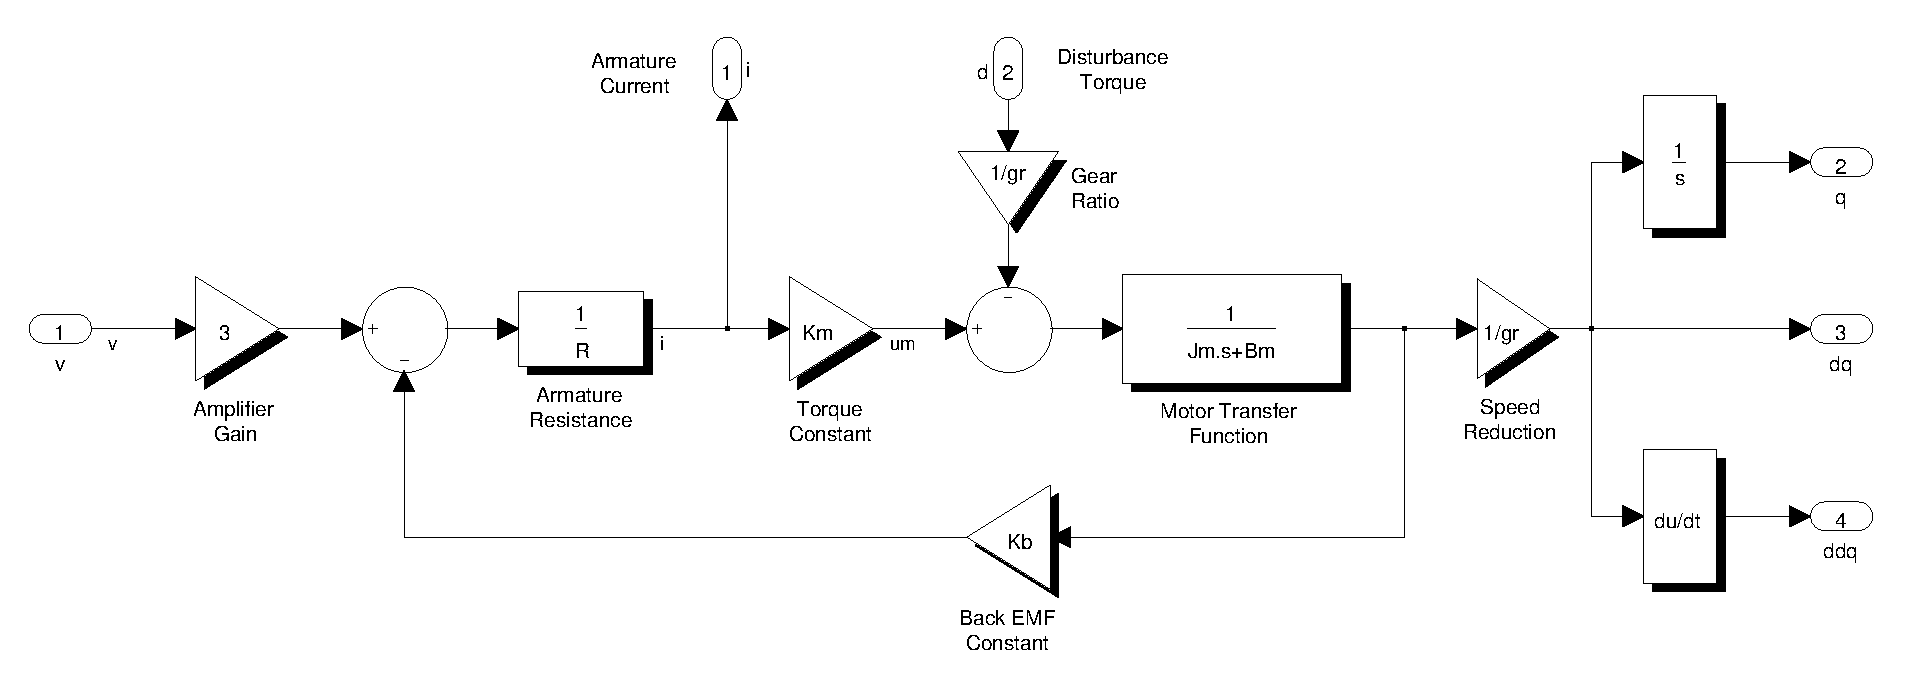
\includegraphics[scale=0.55]{fig/experiments/simmodel.eps} 
  	\caption{Subsystem from Figure~\ref{fig:parallelmodels} used to target the simulated environment with voltage control signal.}
	\label{fig:simmodel}
\end{figure}

% section hil_architecture (end)

\section{Single DOF Validation} % (fold)
\label{sec:1dof_validation}
\Incomplete
% section 1dof_results (end)

\section{Motion Control Validation} % (fold)
\label{sec:motion_control_validation}
\Incomplete
% section motion_control_results (end)

\section{Discussion} % (fold)
\label{sec:experiments_discussion}
\Incomplete
% section discussion (end)

% chapter experiments (end)